%%%%%%%%%%%%%%%%%%%%%%%%%%%%%%%%%%%%%%%%%
% Journal Article
% LaTeX Template
% Version 1.4 (15/5/16)
%
% This template has been downloaded from:
% http://www.LaTeXTemplates.com
%
% Original author:
% Frits Wenneker (http://www.howtotex.com) with extensive modifications by
% Vel (vel@LaTeXTemplates.com)
%
% License:
% CC BY-NC-SA 3.0 (http://creativecommons.org/licenses/by-nc-sa/3.0/)
%%%%%%%%%%%%%%%%%%%%%%%%%%%%%%%%%%%%%%%%%

%----------------------------------------------------------------------------------------
%	PACKAGES AND OTHER DOCUMENT CONFIGURATIONS
%----------------------------------------------------------------------------------------

\documentclass[twoside,twocolumn]{article}

\usepackage{blindtext} % Package to generate dummy text throughout this template

\usepackage[sc]{mathpazo} % Use the Palatino font
\usepackage[T1]{fontenc} % Use 8-bit encoding that has 256 glyphs
\linespread{1.05} % Line spacing - Palatino needs more space between lines
\usepackage{microtype} % Slightly tweak font spacing for aesthetics

\usepackage[german]{babel} % Language hyphenation and typographical rules

\usepackage[hmarginratio=1:1,top=32mm,columnsep=20pt]{geometry} % Document margins
\usepackage[hang, small,labelfont=bf,up,textfont=it,up]{caption} % Custom captions under/above floats in tables or figures
\usepackage{booktabs} % Horizontal rules in tables

\usepackage{lettrine} % The lettrine is the first enlarged letter at the beginning of the text

\usepackage{enumitem} % Customized lists
\setlist[itemize]{noitemsep} % Make itemize lists more compact

\usepackage{abstract} % Allows abstract customization
\renewcommand{\abstractnamefont}{\normalfont\bfseries} % Set the "Abstract" text to bold
\renewcommand{\abstracttextfont}{\normalfont\small\itshape} % Set the abstract itself to small italic text

\usepackage{titlesec} % Allows customization of titles
\renewcommand\thesection{\Roman{section}} % Roman numerals for the sections
\renewcommand\thesubsection{\roman{subsection}} % roman numerals for subsections
\titleformat{\section}[block]{\large\scshape\centering}{\thesection.}{1em}{} % Change the look of the section titles
\titleformat{\subsection}[block]{\large}{\thesubsection.}{1em}{} % Change the look of the section titles

\usepackage{fancyhdr} % Headers and footers
\pagestyle{fancy} % All pages have headers and footers
\fancyhead{} % Blank out the default header
\fancyfoot{} % Blank out the default footer
\fancyhead[C]{Evolutionäre Optimierungsalgorithmen $\bullet$ MK - Einführung in das wissenschaftliche Arbeiten} % Custom header text
\fancyfoot[RO,LE]{\thepage} % Custom footer text

\usepackage{titling} % Customizing the title section

\usepackage{hyperref} % For hyperlinks in the PDF

\newcommand{\e}[1]{\times 10^{#1}}

\usepackage{graphicx}

\usepackage{amsmath}

\usepackage{csquotes}

%----------------------------------------------------------------------------------------
%	TITLE SECTION
%----------------------------------------------------------------------------------------

\setlength{\droptitle}{-4\baselineskip} % Move the title up

\pretitle{\begin{center}\Huge\bfseries} % Article title formatting
\posttitle{\end{center}} % Article title closing formatting
\title{Evolutionäre Optimierungsalgorithmen} % Article title
\author {
	\textsc{Federico Ramírez Villagrana} \\[1ex]
	\normalsize Universität Hamburg \\
	\normalsize Methodenkompetenz - Einführung in das wissenschaftliche Arbeiten \\
	\normalsize Dozent: Dr. Andreas Günther
}
\date{} % Leave empty to omit a date
\renewcommand{\maketitlehookd}{%
\begin{abstract}
\noindent In diesem Paper wird es darüber diskutiert, sowohl was Optimierung ist und warum ist es schwer, als auch was evolutionärer Algorithmen (EA) sind und wie, warum,  und wann sind sie hilfreich in dem Optimierung-Bereich. Es wird auch im Detail erklärt, wie EA funktionieren und warum sind sie als teil des künstlichen Intelligenz betrachtet. Es werden auch einige bekannten EA präsentiert und oberflächlich erklärt. Am ende wird es darüber diskutiert, was für Vor- und Nachteile die EA haben.
\end{abstract}
}

%----------------------------------------------------------------------------------------

\begin{document}

% Print the title
\maketitle

%----------------------------------------------------------------------------------------
%	ARTICLE CONTENTS
%----------------------------------------------------------------------------------------

\section{Einleitung}

\lettrine[nindent=0em,lines=3]{D} as Problem des Handlungsreisenden (engl. traveling salesman problem oder TSP) ist ein sehr bekanntes und studierte Problem in dem Informatik-Bereich und es geht wie folgendes:\par
Es muss eine Reihenfolge für den Besuch mehrerer Orte so gewählt sein, dass keine Station außer der ersten mehr als einmal besucht wird, die gesamte Reisestrecke des Handlungsreisenden möglichst kurz, und die erste Station gleich der letzten Station ist. \cite{wiki_tsp}\par
Sei $n$ die Anzahl der Stationen, es gibt $(n-1)!$ mögliche Lösungen für das TSP. Das heißt, dass für $n=4$ es gibt $6$ mögliche Lösungen. Es ist nicht schwer einen brute-force \footnote{Auch Exhaustionsmethode, ist eine Lösungsmethode für Probleme, die auf dem Ausprobieren aller möglichen (oder zumindest vieler möglicher) Fälle beruht. \cite{wiki_brute_force}} Ansatz zu verfolgen für ein Problem, das nur 6 Lösungen hat. Aber wenn $n=50$ es gibt circa $6,1\e{62}$ Lösungen.\par
Folgendes ist hilfreich, um diese Anzahl in eine Perspektive zu setzen: Das Universum ist circa 15 Milliarde Jahre alt, das ist $4,7\e{17}$ Sekunden. Wenn es eine Billion Rechner gäbe, die jeder einzeln seit dem Anfang des Universums eine Billion Lösungen pro Sekunde berechnete, bisher wären nur $4,7\e{41}$ Lösungen berechnet worden.\par
Das TSP ist nur ein Beispiel von vielfältigen Probleme, die zu den kombinatorischen Problemen gehören, das heißt, Probleme für die einfach keine brute-force Ansatz möglich ist. Es ist in diesem Fall, dass evolutionärer Algorithmen (EA) hilfreich sind.\par
EA sind eine gute Werkzeug um gute Lösungen zu finden. Natürlich können wir nicht sicher sein, dass wir das beste Lösung gefunden haben, außer wenn wir jeder mögliche Lösungen berechnen haben. Aber wie es mit dem TSP-Beispiel gezeigt ist, es ist nicht immer möglich, alle mögliche Lösungen zu finden.

%------------------------------------------------

\section{Stand der Forschung}

Todo

%------------------------------------------------

\section{Optimierung}

\lettrine[nindent=0em,lines=3]{I} n dem Mathematik-Bereich, Optimierung bedeutet die Findung von Parametern eines Systems, die ein bestmögliches Ergebnis erzielen. \cite{wiki_optimierung} Wir können diese Findung von Parametern auch wie Folgendes definieren: Die Auswahl von die bestmögliche Lösung eines Problems von einer Menge mögliche Lösungen.\par
In Optimierungsprobleme wird eine Zielfunktion (engl. objective function) definiert, die entweder maximiert oder minimiert werden soll. Die Zielfunktion wird \enquote{Kosten-Funktion} oder \enquote{Fitness-Funktion} in Minimierung- und Maximierungsprobleme bzw. genannt.\par
Sei $f(x)$ ein Zielfunktion, $x$ ist ein Vektor und wird \enquote{Entscheidungsvariable} genannt. Die Anzahl von Elementen in $x$ wird die Dimension des Problems genannt.
Die Domäne der Zielfunktion repräsentiert die mögliche Lösungen des Problems. \par
Das Ziel der Optimierung ist es denn, die bestmögliche Lösung des Problems zu finden, das heißt, einen Wert für die Entscheidungsvariable zu finden, sodass die Zielfunktion einen maximal bzw. minimal Wert ergibt.\par
Es gibt verschiedene Klassifizierungen oder Arten von Optimierung:

\begin{itemize}
\item{Eingeschränkt Optimierung.}\\
Die Entscheidungsvariable kann nicht irgendwelcher Wert nehmen. Es gibt Einschränkungen dafür.\\
\item{Multi-objective Optimierung.}\\
Das Problem besteht aus vielfältigen, voneinander unabhängig Zielfunktionen.\\
\item{Multi-modal Optimierung.}\\
Die Zielfunktion(en) hat/haben mehrere Minima bzw. Maxima. Abbildung \ref{fig:rastrigin} zeigt eine multi-modale Funktion.
\end{itemize}

\begin{figure}[h]
\caption{ Rastrigin function. Quelle: \url{https://commons.wikimedia.org/wiki/File:Rastrigin_function.png}}
\label{fig:rastrigin}
\centering
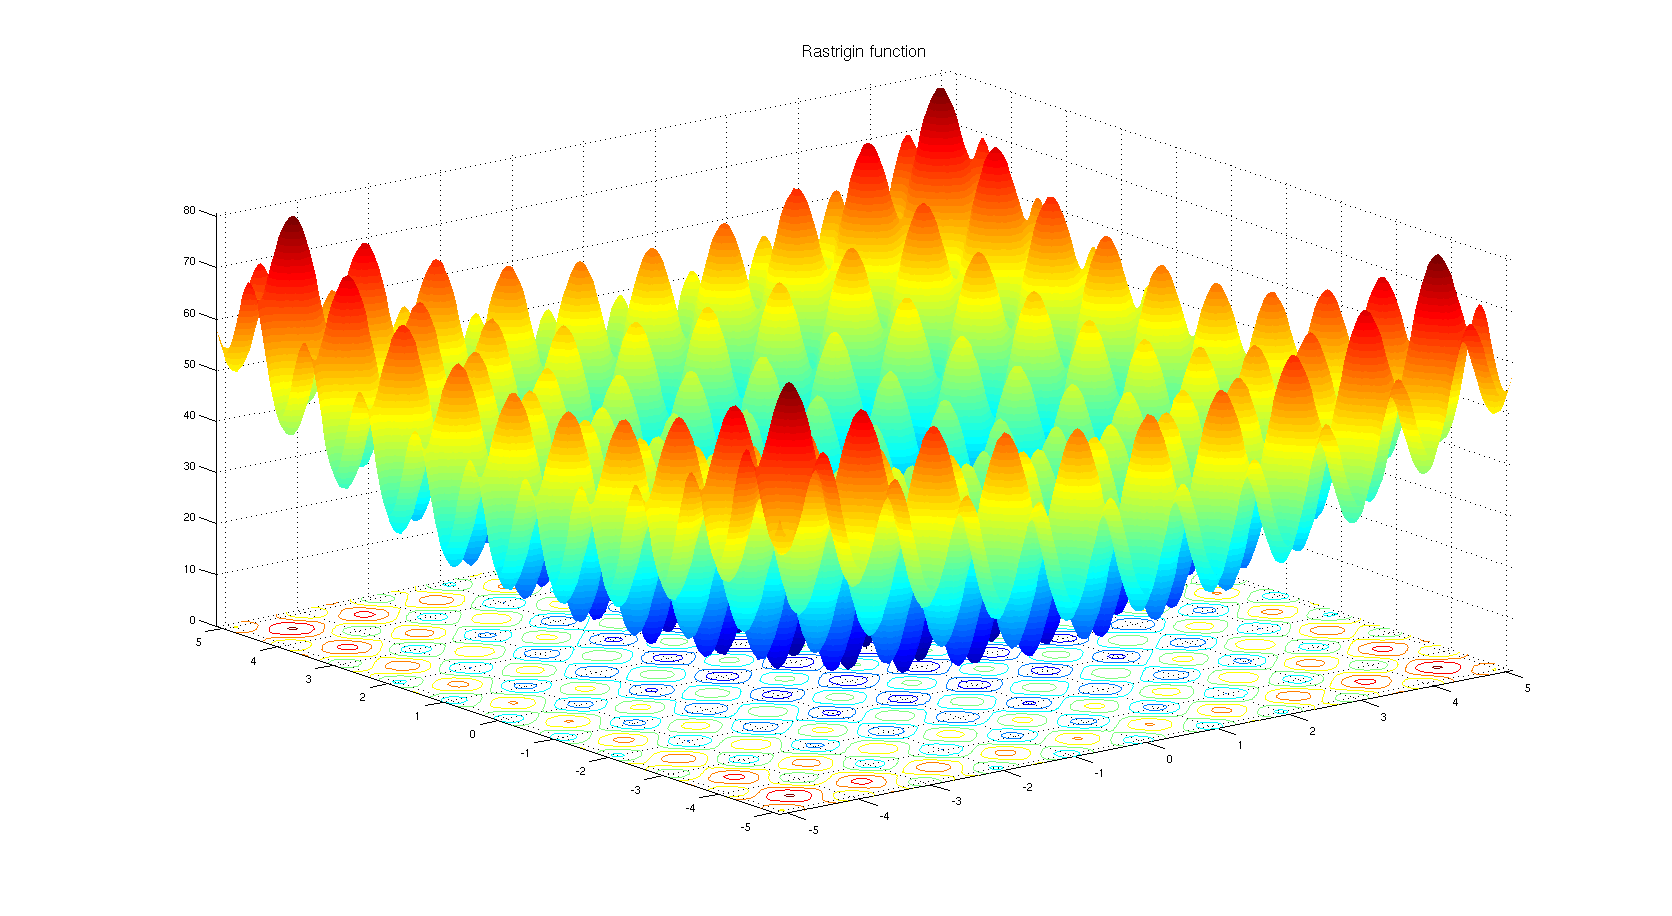
\includegraphics[width=0.5\textwidth]{images/rastrigin_function.png}
\end{figure}

Eine der wichtigste und schwerste Teile der Optimierung ist es, eine geeignete Zielfunktion zu definieren, die alle die wichtige zu optimieren Faktoren berücksichtigt.
Probleme im wirklichen Leben sind normalerweise eingeschränkt, multi-Objective und multi-modale, oder mit eine hoch Anzahl von Dimensionen. Wegen diesen Eigenschaften der Zielfunktionen und der Optimierungsprobleme ist es schwer eine gute Lösung mittels traditionelle Vorgänge  zu finden. EA sind aber eine gute Möglichkeit, um diese Art von Probleme in angemessene Zeit zu lösen.

%------------------------------------------------

\section{Was ist ein evolutionärer Algorithmus?}

\lettrine[nindent=0em,lines=3]{D} er EA-Bereich ist ziemlich neu, deswegen gibt es bisher keine allgemein akzeptierte Definition von evolutionäre Algorithmus.\par
EA sind zwar als Teil des künstliche Intelligenzes (KI) betrachtet, aber genau wo sie in Verbindung mit anderen KI-Methoden stehen, und was die EA-Bereich beinhaltet, ist von dem Autor abhängig. Abbildung \ref{fig:metaheuristics} zeigt eine von mehrere mögliche Klassifikationen von KI-Methoden in Bezug auf Metaheuristics (welche über den Rahmen dieses Papiers hinausgehen).\\

\begin{figure}[h]
\caption{ Klassifikation von Metaheuristics. Quelle: \url{https://en.wikipedia.org/wiki/File:Metaheuristics_classification.svg}}
\label{fig:metaheuristics}
\centering
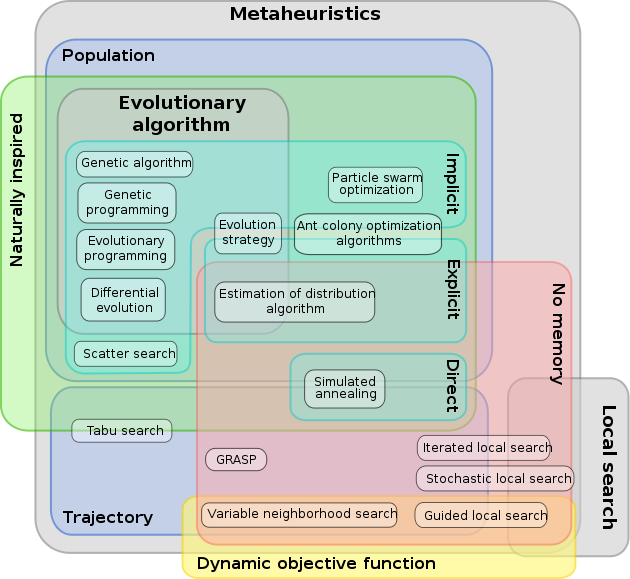
\includegraphics[width=0.5\textwidth]{images/metaheuristics_classification.png}
\end{figure}

In Abbildung \ref{fig:metaheuristics} können wir es auch sehen, wie der Autor betrachtet Particle Swarm Optimization (PSO) und Ant Colony Optimization (ACO) nicht als EA, trotzdem gibt es andere Autoren (wie z. B. \cite{wiley_evolutionary}), die diese Algorithmen genau für EA halten.

In diesem Paper wird folgende Definition für EA genommen: Ein Algorithmus, der die Lösung eines Problems durch viele Iterationen entwickelt    .

\subsection{Eigenschaften der EA}
Folgende sind die Hauptmerkmale der EA:

\begin{itemize}
\item{Eine Zielfunktion.}\\
\item{Eine - so genannte - Bevölkerung von mögliche Lösungen.}\\
Eine Menge von Darstellungen der Lösungen (Elemente der Domäne der Zielfunktion) des Problems, die mittels der Algorithmus und mehrere Iterationen verarbeitet und hoffentlich verbessert werden.\\
\item{Vorgänge, die die Elementen der Bevölkerung betreffen und verändern.}\\
Diese können der Algorithmus selber oder ein äußern Verfahren sein.
\end{itemize}

Die meisten EA sind aus die Natur inspiriert, das heißt, dass Wissenschaftler Ereignisse, Systeme, und Mechanismen von der Natur beobachten und danach versuchen einigermaßen, sie mit Algorithmen zu reproduzieren. Sie werden \enquote{evolutionär} genannt, denn sie sind ursprünglich aus der Evolution inspiriert. \cite{holland_ga}\par

Wie vorher gesagt, EA sind als Teil des KI betrachtet, das ist weil EA emulieren Eigenschaften von intelligente Systeme aus der Natur.\par

Nach \cite{wiley_evolutionary} sind die folgende Eigenschaften notwendig, um ein System als intelligent zu betrachten:

\begin{itemize}
\item{Adaptation.}\\
Ein intelligentes System muss in hohem Maße an unvorhersehbare Änderungen anpassbar sein. Lernen ist daher unerlässlich.\\
\item{Zufälligkeit.}\\
Obwohl Zufälligkeit meistens als eine schlechte Eigenschaft betrachtet wird, es ist in gewissem Maße notwendig, damit neue Lösungen eines Problems gefunden sein können.\\
\item{Kommunikation.}\\
Eine einzige Ameise ist nicht wirklich als intelligent betrachtet, aber eine Ameisenkolonie ist (dank Kommunikation durch Pheromone) als eine super-intelligent Einheit überlegt.\\
\item{Rückmeldung.}\\
Ein System kann sich nicht anpassen und verbessern, wenn es seine Umgebung nicht erkennen und darauf reagieren kann. Auch um zu lernen, muss ein System seine Fehler (mittels Rückmeldung) erkennen.\\
\item{Erkundung.}\\
Das heißt neue Lösungen finden, neue Wege erkunden.\\
\item{Ausbeutung.}\\
Im Gegenteil zu Erkundung, Ausbeutung heißt, schon bekannten Lösungen und Wege ausnutzen.
\end{itemize}

In nächster Sektion werden verschiedene Beispiele von EA gezeigt und in jeder Beispiel wird es erwähnt, welcher Teil des Algorithmuses welche Eigenschaft des Intelligenzes versucht zu emulieren. Es ist auch wichtig zu sagen, dass nicht alle Eigenschaften des Intelligenzes von jeder EA repliziert sind.

%------------------------------------------------

\section{EA Beispiele}

Heutzutage gibt es aber viele EA und jedes Jahr werden neue entwickelt. In dieser Sektion werden nur ein paar der bekanntesten und wichtigsten erwähnt und oberflächlich erklärt.

\subsection{Genetic Algorithmen - GA}
Genetic Algotihmen (GA) sind ursprünglich in \cite{holland_ga} präsentiert und danach in \cite{goldberg_ga} weiter entwickelt. Der Name \enquote{Genetic Algorithms} bezieht sich mehr auf eine Familie von Algorithmen als auf einen einzigen Algorithmus.\par
GA sind die erste vorgestellte, bekannteste, und am meistens verwendeten EA. Ursprünglich waren sie dafür entwickelt, um adaptierbare Systeme zu studieren. Sie sind Simulationen der natürlichen Selektion. Daher sind sie genau aus der Evolution inspiriert.\par
Es gibt sechs Hauptteile eines GAs:

\begin{enumerate}
\item{Codierung der Lösungen.}\par
Als erstes muss man eine geeignete Codierung für die mögliche Lösungen finden. Das heißt, eine Darstellung für die Lösungen finden, die einfach zu verarbeiten ist. Eine die am meistens verwendeten Codierungen ist eine Bit-Folge. In dieser Codierung jedes Bit wird \enquote{Gen} genannt.
\item{Ursprüngliche Bevölkerung.}\par
Eine ursprüngliche Bevölkerung muss initialisiert werden. Diese Initialisierung kann entweder zufällig oder auf vorher Kenntnisse basiert sein. Wie viele Elementen die Bevölkerung hat, ist ein wichtige Parameter. Je mehrere Elemente desto eine bessere Wahrscheinlichkeit, um gute Lösungen zu finden.
\item{Fitnessfunktion.}\par
Die Zielfunktion des Problems.\par
Der Wert, den die Zielfunktion ergibt, wenn sie für den Wert ausgewertet wird, den ein Element der Bevölkerung darstellt, wird die \enquote{Fitness} des Elements genannt.
\item{Auswahl von Einzelnen.}\par
Zwei Elemente der Bevölkerung werden ausgewählt, um ein neue Element herzustellen. Das Verfahren um die Elemente auszuwählen kann entweder zufällig oder auf die Fitness der Elemente basiert sein. Die ausgewählte Elemente werden \enquote{Eltern}' genannt.
\item{Crossover.}\par
Dies ist das wichtigste Teil eines GA. Es definiert wie das neue Element aus die Eltern erstellt wird. Das heißt, welche Gene wird das neue Element von jeden Elternteil erben.
\item{Mutation.}\par
Einige zufälligerweise-ausgewählt neue erstellt Elemente werden mutiert sein. Das heißt, dass einige Bits gekippt werden. Welche Elemente werden mutiert und wie viele und welche Bits werden gekippt, kann mittels verschiedene Verfahren entscheidet werden.
\end{enumerate}

\begin{figure}[h]
\caption{ Wesentlich genetic Algorithmen pseudo-Code. Quelle: \cite{wiley_evolutionary}}
\label{fig:ga_pseudo}
\centering
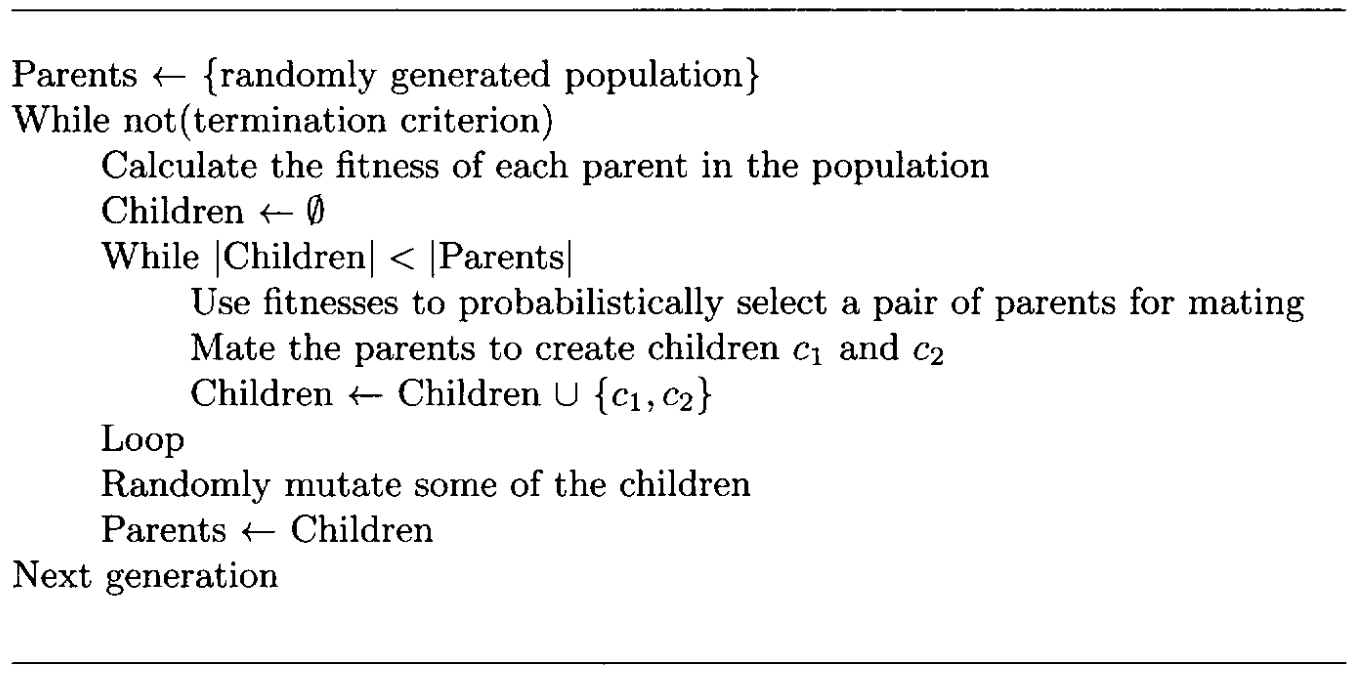
\includegraphics[width=0.5\textwidth]{images/ga_pseudo.png}
\end{figure}

Bei GA ist Adaptation anwesend, denn diese Art von Algorithmen ist Problem-unabhängig. Mit anderen Wörter, wenn es eine geeignete Darstellung der Lösungen gibt, kann das Problem mit GA optimiert wird.\par
In Teil 2 sowie in Teile 4 bis 6 kann Zufälligkeit verwendet werden, je nachdem welche Verfahren bzw. ausgewählt werden.\par
In der Mutation-Teil, eine hoch Wahrscheinlichkeit um Elemente zu mutieren heißt viel Erkundung und weniger Ausbeutung und umgekehrt.

\subsection{Particle Swarm Optimization - PSO}
Particle Swarm Optimization (PSO) Algorithmus ist ursprünglich in \cite{kennedy_pso} und in \cite{shi_pso} präsentiert.\par
PSO ist auf menschliches soziales Verhalten basiert. \cite{eberhart_pso} Genauer,  PSO basiert auf der Beobachtung von Gruppen von Individuen, die zusammenarbeiten, um nicht nur ihr kollektives Verhalten in einer bestimmten Aufgabe zu verbessern, sondern auch ihr individuelles Verhalten zu verbessern.\par
Die Grundideen hinter PSO sind wie folgendes:

\begin{itemize}
\item Es gibt eine Menge Partikeln, die sich mit einer beliebigen Geschwindigkeit durch den Suchraum bewegen.
\item Der Suchraum ist in \enquote{Nachbarschaften} mit einer beliebigen gleichen Größe unterteilt.
\item Jeder Partikeln speichert sowohl die beste Position, die sie im Suchraum besucht hat, als auch die beste Position, die ihre Nachbarn erreicht haben.
\item Beide die Partikels beste Position und ihre Nachbarns beste Positionen beeinflussen die Partikels Geschwindigkeit.
\end{itemize}

\begin{figure}[h]
\caption{ Wesentlich PSO Algorithmus pseudo-Code. Quelle: \cite{wiley_evolutionary}}
\label{fig:pso_pseudo}
\centering
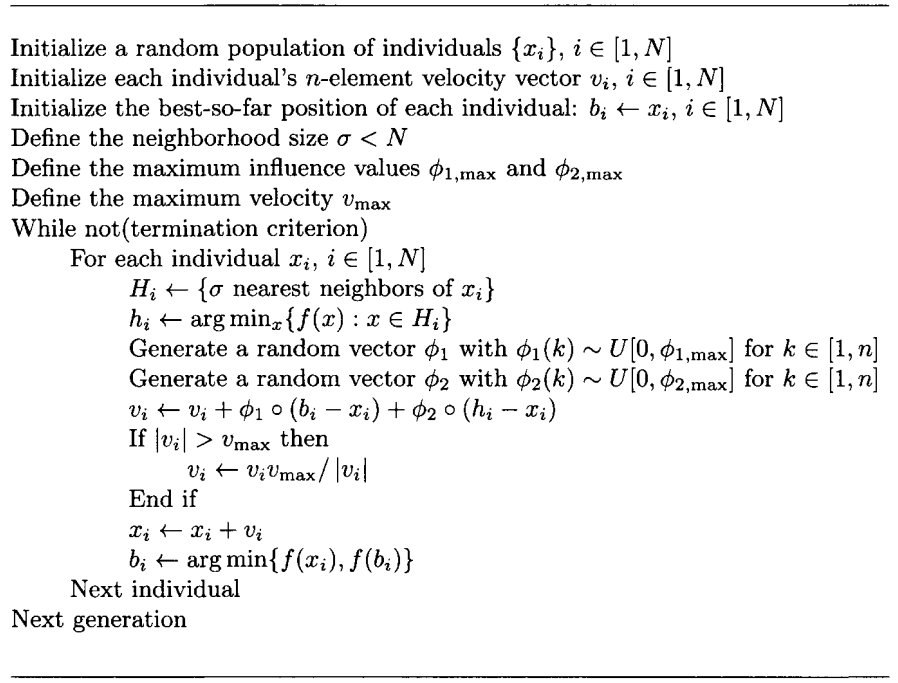
\includegraphics[width=0.5\textwidth]{images/pso_pseudo.png}
\end{figure}

In PSO können die Geschwindigkeiten der ersten Bevölkerung zufällig initialisiert werden. Daher haben wir ein Element der Zufälligkeit.\par
Da die Partikeln die beste bisher erreichte Positionen ihrer Nachbarn kennen müssen, gibt es auch Kommunikation.\par
Die Tatsache, dass die beste bisher erreichte Positionen die Geschwindigkeit der Partikel beeinflussen, zeigt Rückmeldung. In welche Ausmaß wird die Partikel beeinflusst, kann entweder Erkundung oder Ausbeutung fördern.

\subsection{Differential Evolution - DE}
Todo

%------------------------------------------------

\section{Diskussion}

Todo

%------------------------------------------------

\section{Fazit}

Todo

%----------------------------------------------------------------------------------------
%	REFERENCE LIST
%----------------------------------------------------------------------------------------

\renewcommand{\refname}{Quellenverzeichnis}
\bibliographystyle{alpha} %unsrtnat

\bibliography{quellenverzeichnis}

%----------------------------------------------------------------------------------------

\end{document}
